
\section{Overview of the Silicon Tracking System (STS)}
All semiconductor based detector systems include very similar functions. The signals from the detector channels have to be amplified and processed for storage and analysis. The silicon sensors, analog-digital converter and all the necessary support structures are often referred to as a detector module. Nevertheless, there are many parameters that have to be optimized in order to achieve the detector performance. 

The physics observables together with the foreseen accelerator specifications mentioned in the previous chapter define the requirements for the detector system. The \gls{STS} is designed to provide track reconstruction and momentum determination of the charged particles. The detector has to work with ion beam energies from 2 to 14 AGeV (protons 39 GeV). In addition to that, a very high interaction rate 10~MHz results in up to 700 tracks per central Au+Au collisions. The \gls{STS} extends more than \SI{1}{\metre} downstream of the target and will be installed in a volume of \SI{3}{\square\metre}. 

In order to achieve physics goals, \gls{STS} has to address the following:
\begin{itemize}
    \item  aperture - the aperture of the whole experiment is expected to cover polar angles from \SI{2}{\degree} up to \SI{25}{\degree}. This range corresponds to center-of-mass rapidity close to the beam rapidity. 
    \item spatial resolution - a single-hit resolution of about \SI{20}{\micro\metre} in X direction and \SI{120}{\micro\metre} in Y, 
    \item single-hit efficiency - the detector layer should provide almost 100\% detection efficiency. The damaging effect of the radiation, implies that the \footnote{ratio of the most probable amplitude for a minimum ionizing particle divided by the root mean square of the single strip noise}{signal-to-noise} ratio needs to be over 10. Having that, the track reconstruction efficiency should exceed 95\% for particle momenta larger than 1~GeV/c. 
    \item momentum resolution - it's mainly influenced by the material budget of the system. The \gls{STS} is designed with the aim to avoid excessive multiple scattering. It is achieved by placing the electronics, mechanical infrastructure and cooling outside the active area. For the \gls{STS} the momentum resolution of $\Delta p/p = 1.5\%$ is foreseen. 
    \item radiation hardness - the silicon sensors and the electronics need to withstand the total dose of 10~kGy~\cite{Heuser:54798}, 
    \item hit rates and readout - the hit rates of charged particles for the inner-most silicon sensors (10~MHz per $\mathrm{cm^{2}}$ provide the requirements for the readout system (signal shaping time, number of readout channels etc.)
\end{itemize}

A simplified CAD drawing of the \gls{STS} is presented in Figure~\ref{fig_STS}. 

\begin{figure}[!h]
\centering
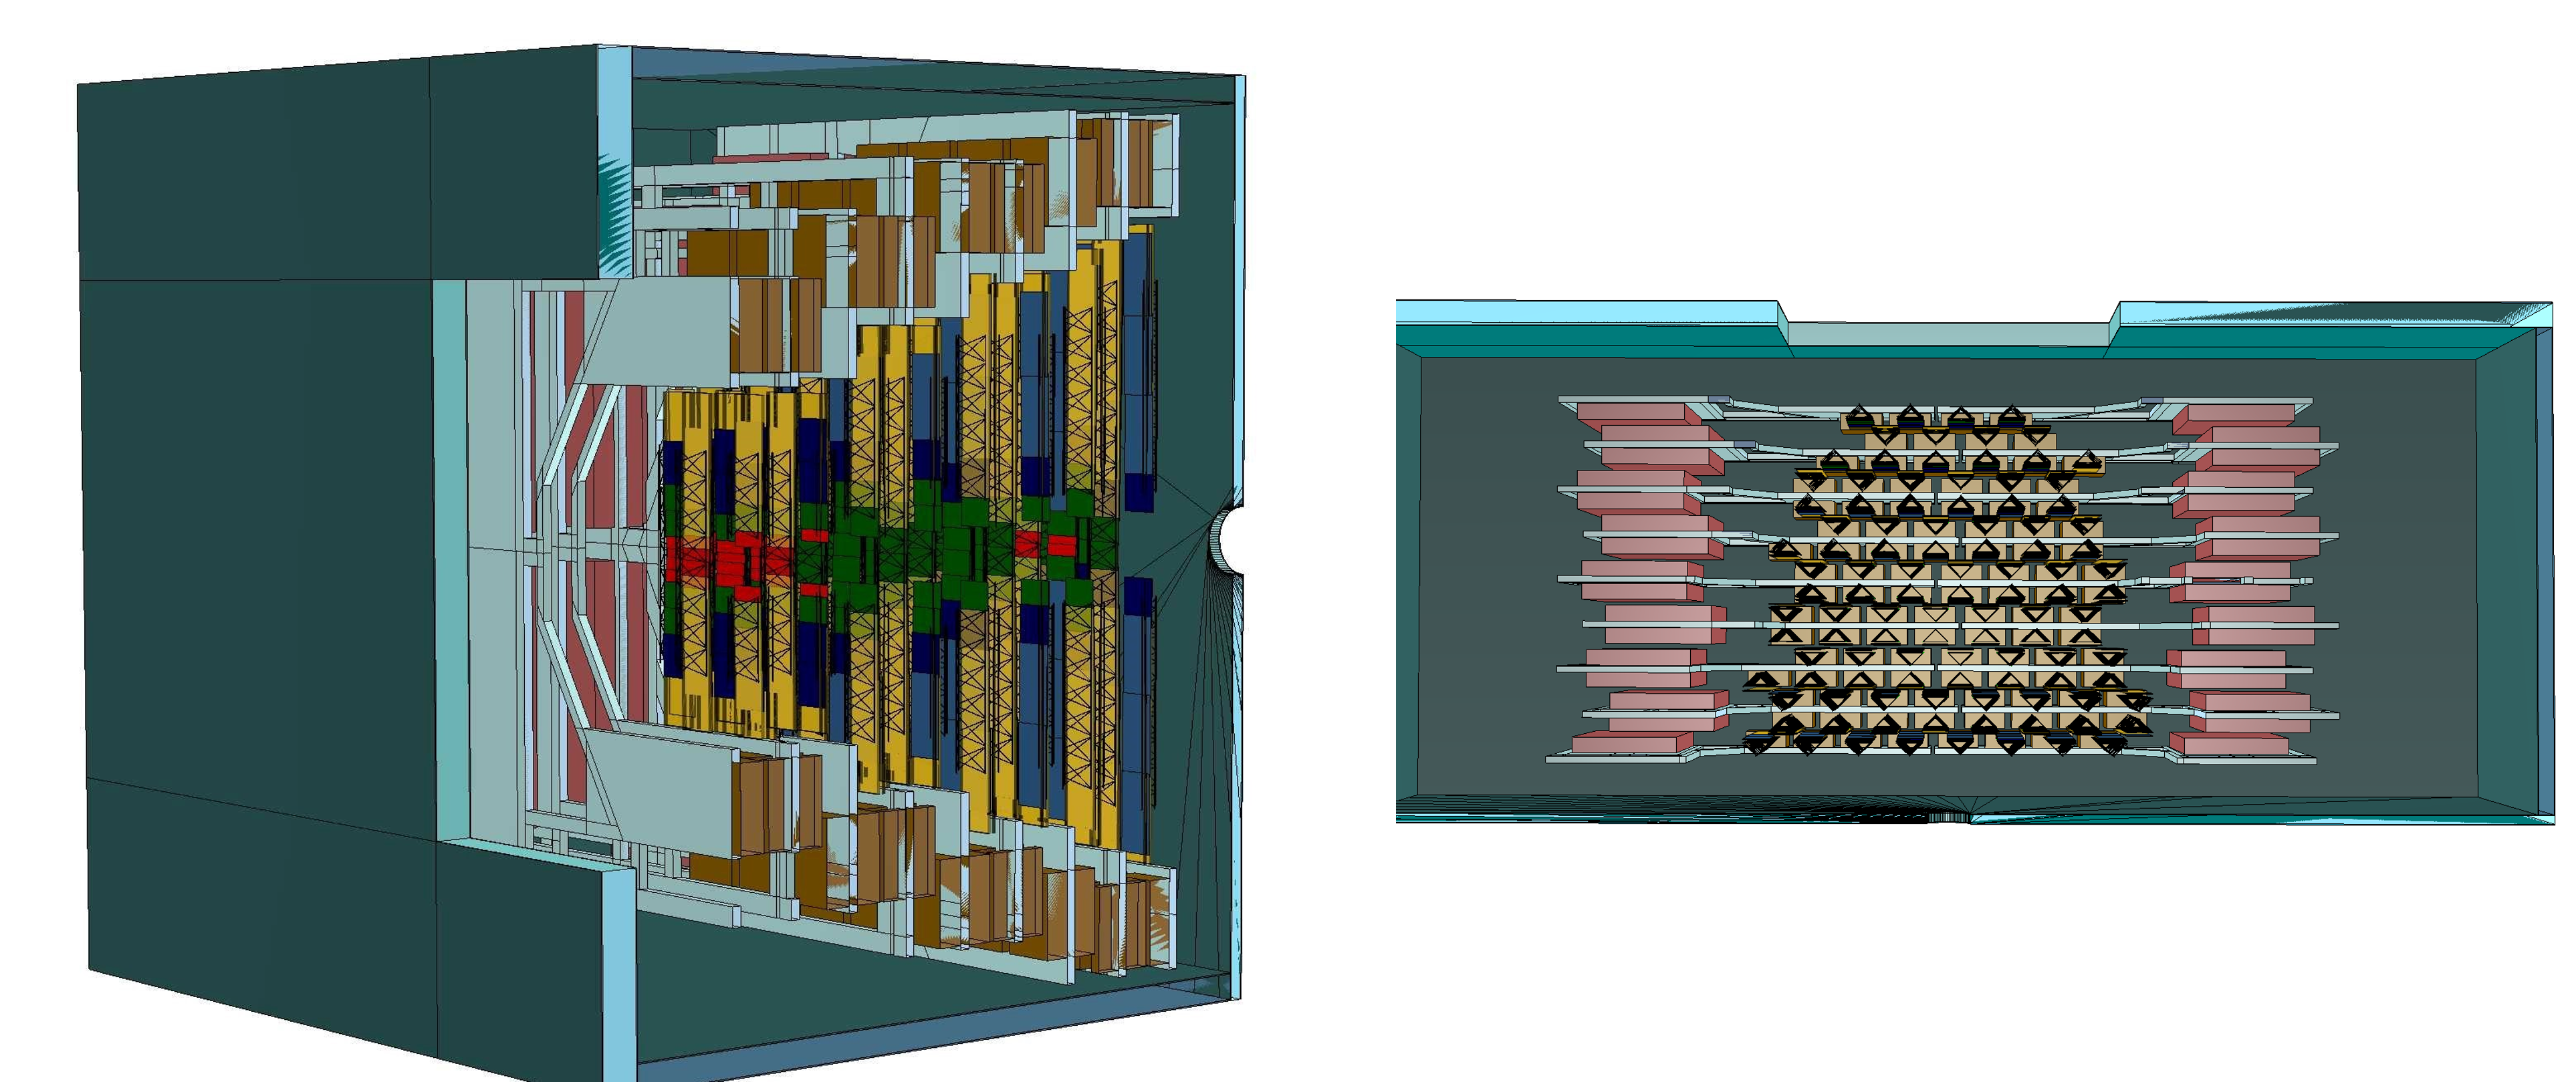
\includegraphics[width=0.85\columnwidth]{Chapter2/images/STS.png}
\caption{A simplified geometry of the Silicon Tracking System. The 8 tracking stations cover the polar angle from \SI{2}{\degree} up to \SI{25}{\degree}.}
\label{fig_STS}
\end{figure}

The detector consists of 876 detectors modules. A module is composed of double-sided silicon microstrip sensors, ultralight microcables (of up to 50~cm length) and Front End Boards (\gls{FEB}) populated with ASICs (STS-XYTER) glued on the fins. The modules are distributed on carbon fiber support-structures which populate C-frames~\cite{progress_report_2016}. Two C-frames form a tracking station of \gls{STS}.  Figure~\ref{fig_assembly} depicts a simplified assembly workflow of \gls{STS}.
The modules are produced in 166 variants, which differ in sensors size, micro-cable length and the orientation of the Front End Electronics~(\gls{FEE}).  
\newpage
\begin{figure}[!h]
\centering
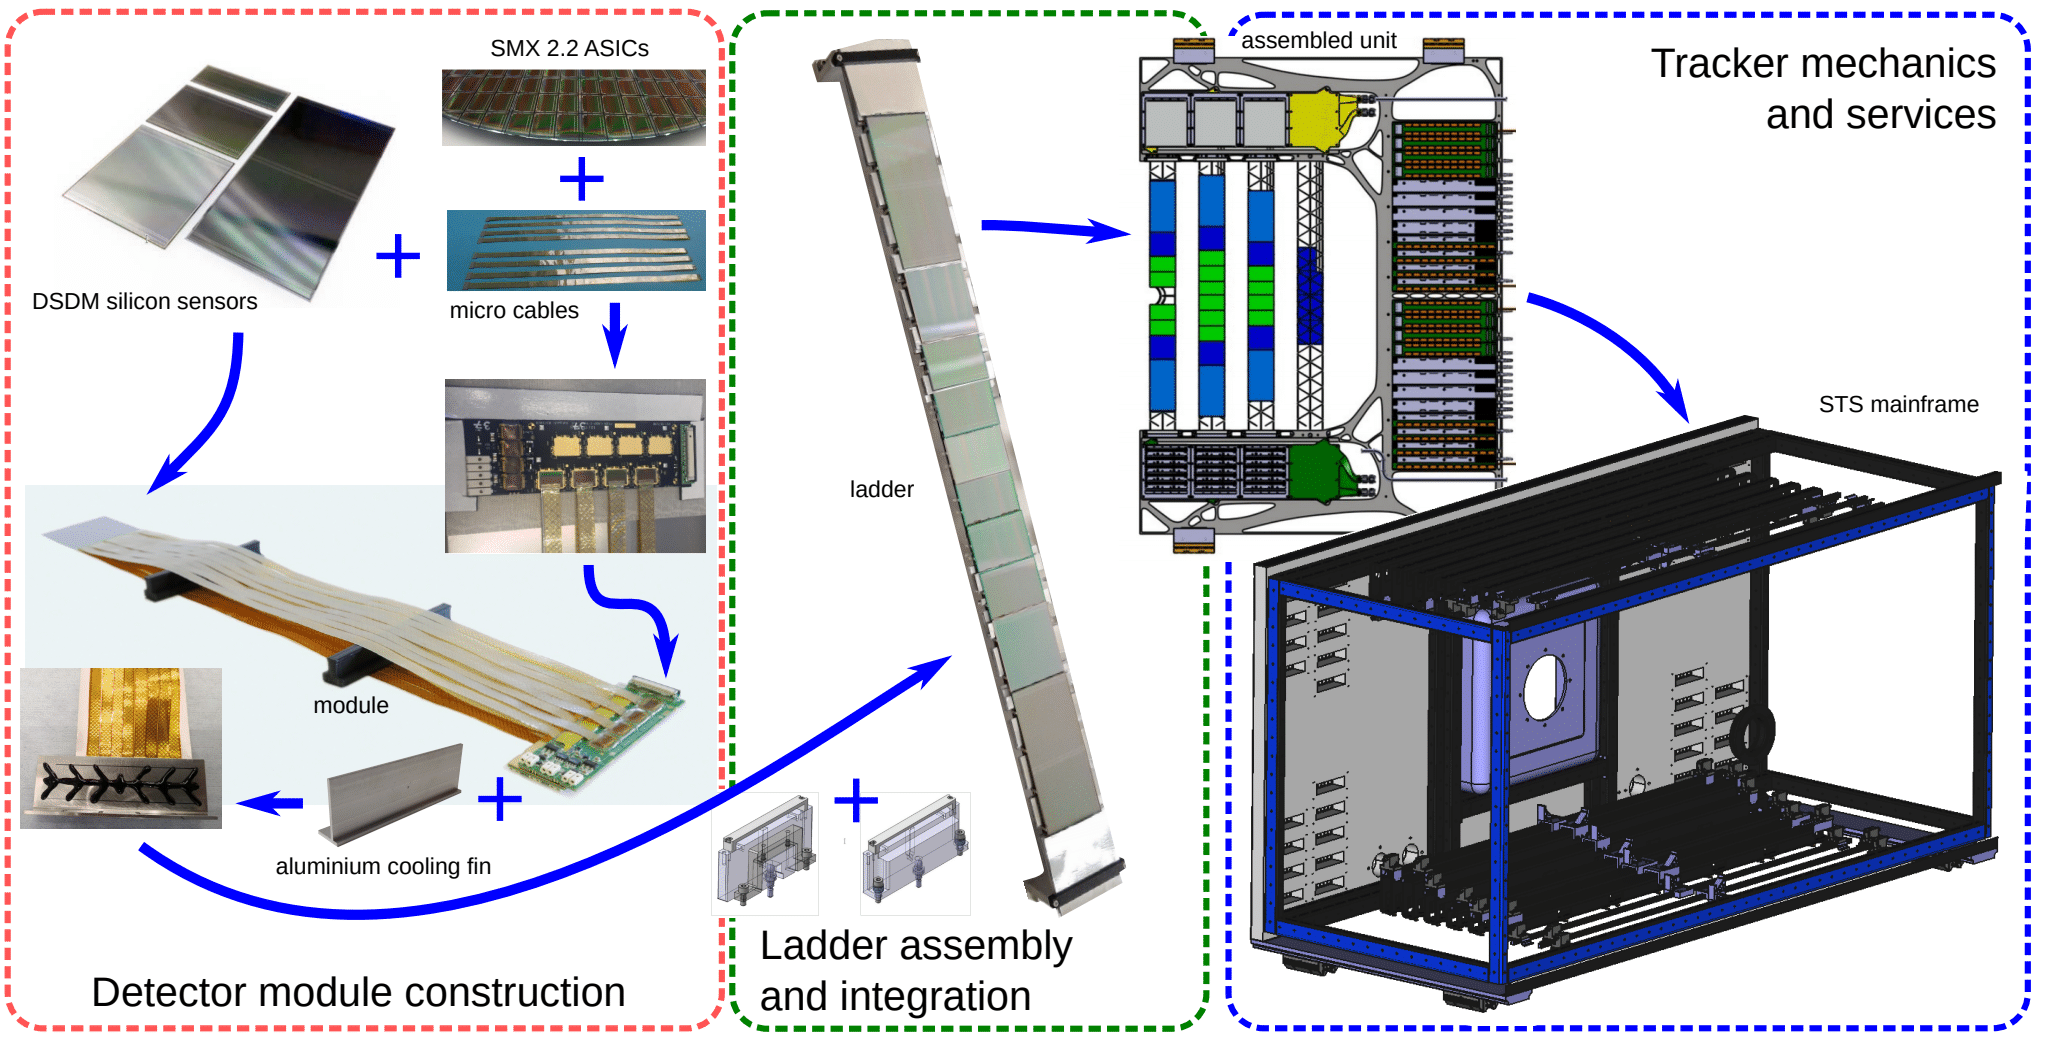
\includegraphics[width=1\columnwidth]{Chapter2/images/assembly_sequence.png}
\caption{A simplified assembly workflow of the \gls{STS}. The silicon sensors are connected to the ASICs on the \glspl{FEB} via microcables. The modules are assembled into carbon fiber ladders which form a C-frame. (Private information from M. Teklishyn)}
\label{fig_assembly}
\end{figure}

%The evolution of different experimental setups constructed for the purpose of testing components of the \gls{STS} is depicted in Figure \ref{fig_evolution_STS}. 

%\begin{figure}[!h]
%\centering
%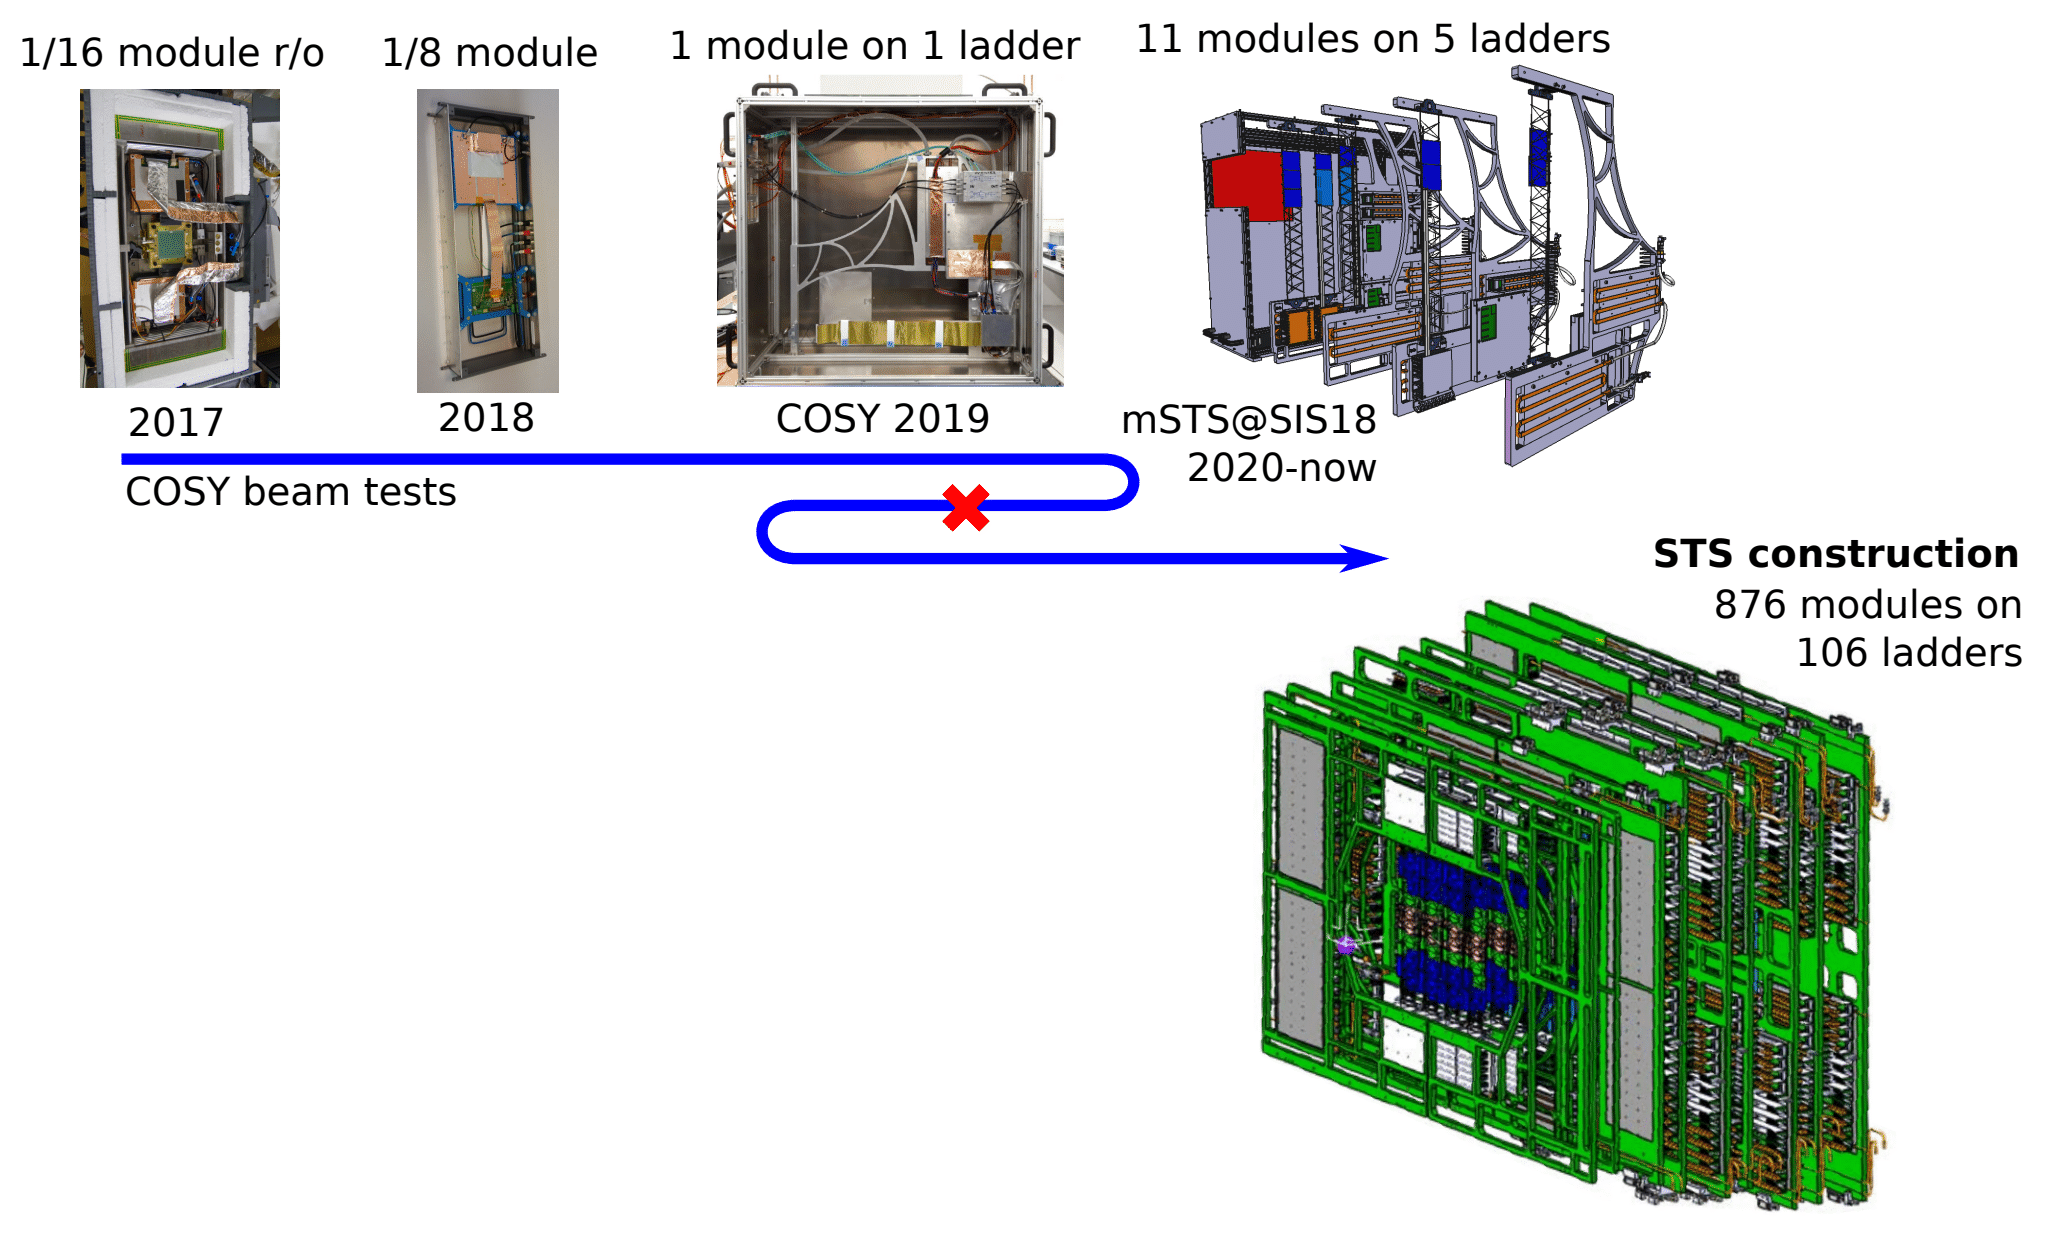
\includegraphics[width=0.95\columnwidth]{Chapter2/images/evolution_sts_new.png}
%\caption{Evolution of the test setups towards \gls{STS}. (Private information %from M. Teklishyn)}
%\label{fig_evolution_STS}
%\end{figure}


That cable design is comparable to \SI{213}{\micro\metre} of silicon for a single detector module.




\subsection{Role of the semiconductors based detector}

Semiconductors can be considered as ionization chambers, which are supplemented with a pair of electrodes and applied external voltage. The radiation passing through the volume of a sensor may result in forming an electron and hole pair. Figure~\ref{fis_si} shows an example of implementing segmented electrodes to determine the particle position. 

\begin{figure}[!h]
\centering
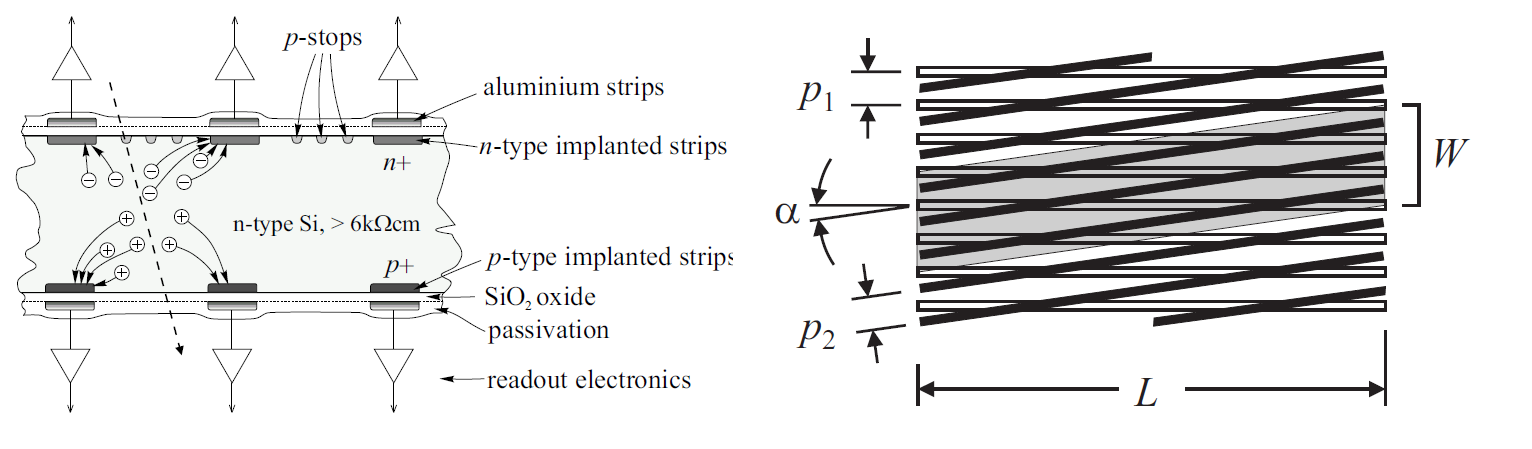
\includegraphics[width=1\columnwidth]{Chapter2/images/silicons.png}
\caption{The segmented electrode enables defining the particle position (left). The segmented second set of strips enables two-dimensional position sensing. The right scheme depicts the strips oriented at a small angle, which aims to reduce fake hits~\cite{Spieler}.}
\label{fig_si}
\end{figure}

Apart from microstrip sensors, there are also pixel devices which enable determining two-dimensional positions. It can be achieved either by proper segmentation of the electronics or designing the geometry.  


The sensitive volume of a silicon sensor produces the average signal current given by 
\begin{equation}
    Q_{s} = \frac{E}{E_{i}}e
\end{equation}
where E is the absorbed energy, $E_{i}$ is the energy required to form a charge pair. The energy needs to be greater than the bandgap, so that the electron can move to the conduction band. The silicon has a gap of 1.12~eV. Nevertheless, the commonly used ionization energy for silicon is about 3.6~eV. This effect is related to the fact that only about 30\% of the particle's energy is converted into electrical signal, the rest goes into phonon excitation.

\subsection{Double-sided microstrip silicon sensors}
\label{sensors}
The use of microstrip silicon sensors was demonstrated in other experiments around the world. It's design and thickness are primarily dependent on the constraints related to the scaterring and signal.

Information about the temperatures serves not only to ensure detector safety, but also to properly understand the behavior of the silicon sensors. One of the important parameters of the silicon sensor is leakage current, which is strongly correlated with the temperature, as per equation \ref{Sil:temp}~\cite{Hartmann:2017gzy}.

The most important formula which allows for the trackers to be used in particle physics is Bethe-Bloch formula:

\begin{equation}
-\dfrac{\mathrm dE}{\mathrm dx} = 4 \pi N_{a} r_{e}^{2} m_{e} c^{2} z^{2}  \dfrac{Z}{A} \frac{1}{\beta^{2}} [\frac{1}{2}\ln(\frac{2m_{e}\gamma^{2}c^{2} T_{max}}{I^{2}}) - \beta^{2} -  2\frac{\delta(\gamma)}{Z}]
\end{equation}

Where z is the charge of the particle, $T_{max}$ is the maximum kinetic energy that can be imparted to a free electron in a single collision, I is the mean excitation energy, Z the atomic number, A the atomic mass, $N_{A}$ the Avogadro’s number, $m_{e}$ the electron mass, c the speed of light, $r_{e}$ the classical electron radius, $\beta = v/c$ and $\gamma = \frac{1}{\sqrt{1-\square\beta}}$ and $\delta$ density effect correction. It describes the average energy loss of a charged particle in a given medium (for example, gas or a semiconductor). 

Silcon sensors

Radiation damage can be divided into two main groups: bulk and surface damage. The influence of the radiation on the silicon is described by so-called Hamburg model. 

The traversing particles are not only causing the ionization of the lattice, but also interact with the silicon via electromagnetic and strong forces. Atoms can be displaced and create defects. Those defects populate new levels in the band gap, changing the properties of the silicon. That’s why the performance of the silicon sensor will degrade over time, what should also be considered while designing an experiment. 




\begin{equation}
\label{Sil:temp}
    I_{R}(T) \propto T^{2}e^{\frac{-E}{2kT}}
\end{equation}
 By assuming that one of the  temperature sensors at a similar height as the silicon sensors mimics their temperature. This assumption clearly doesn't consider several effects like silicon sensors' self-heating. Nevertheless, it allows us to scale down leakage current to $20\,^{\circ}$C using the equation \ref{Sil:scal}.
 
\begin{equation}
\label{Sil:scal}
    \frac{I_{R}(T_{2})}{I_{R}(T_{1})} = (\frac{T_{2}}{T_{1}})^{2}e^{\frac{-E}{2kT}\frac{T_{1}-T_{2}}{T_{1}T_{2}}}
\end{equation}

\begin{figure}[!h]
\centering
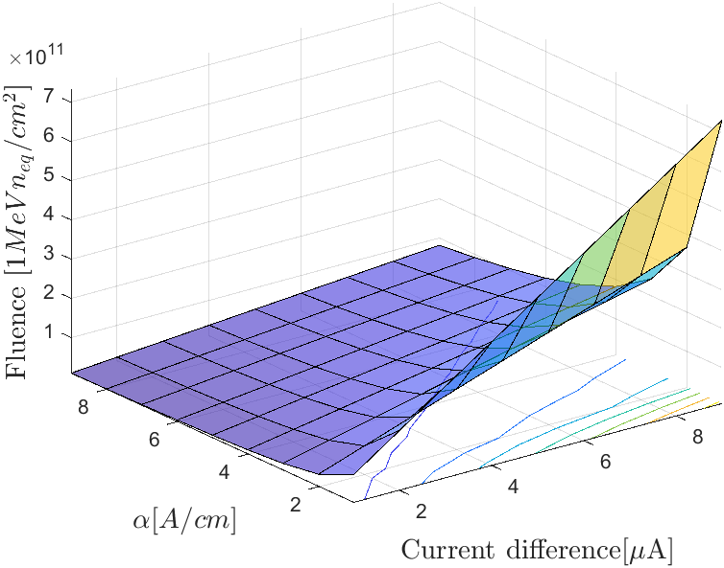
\includegraphics[width=0.65\columnwidth]{Chapter2/images/Leakage_current.png}
\caption{Fluence estimations based on the Hamburg model.}
\label{fig_leakage}
\end{figure}

\begin{figure}[!h]
\centering
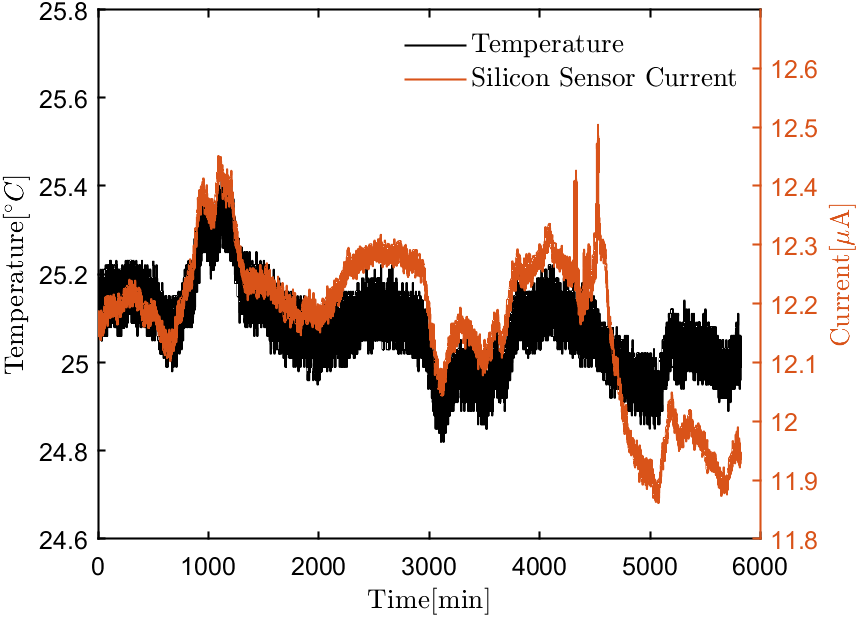
\includegraphics[width=0.65\columnwidth]{Chapter2/images/currenttempnobeam.png}
\caption{The first proposition of the CBM readout chain based on separate DPB and FLIB boards \cite{CRI}}
\label{fig_leakage1}
\end{figure}



\subsection{Module}
\label{module}
 The assembly of the detector is realized stepwise. The whole complex procedure requires utmost care and extremely high precision. Therefore, a proper workflow was developed to address the complexity of the module assembly~\cite{carmen2}.

\subsection{The readout chain of the STS}
\label{readout}
\label{DAQ}
\subsubsection{STS-XYTER}

\subsubsection{Front-end boards (FEB)}

\subsubsection{Readout board (ROB)}

\subsubsection{Common Readout Interface (CRI)}
\subsection{Alternative readout chains for testing purposes}

\subsection{DPB-based readout chain}

\subsection{Tester readout chain}

There are three main readout chains that have been exercised for different detector development activities.  
The readout chain used in the module or FEBs test is built from two components: 
\begin{enumerate}
    \item the Common Readout Board (\gls{CROB}) for data concentration and transport with electrical to optical interface (see figure 
    \item Data Processing Board (DPB) based on the AFCK board (see Fig.
\end{enumerate}

\begin{figure}[!h]
\centering
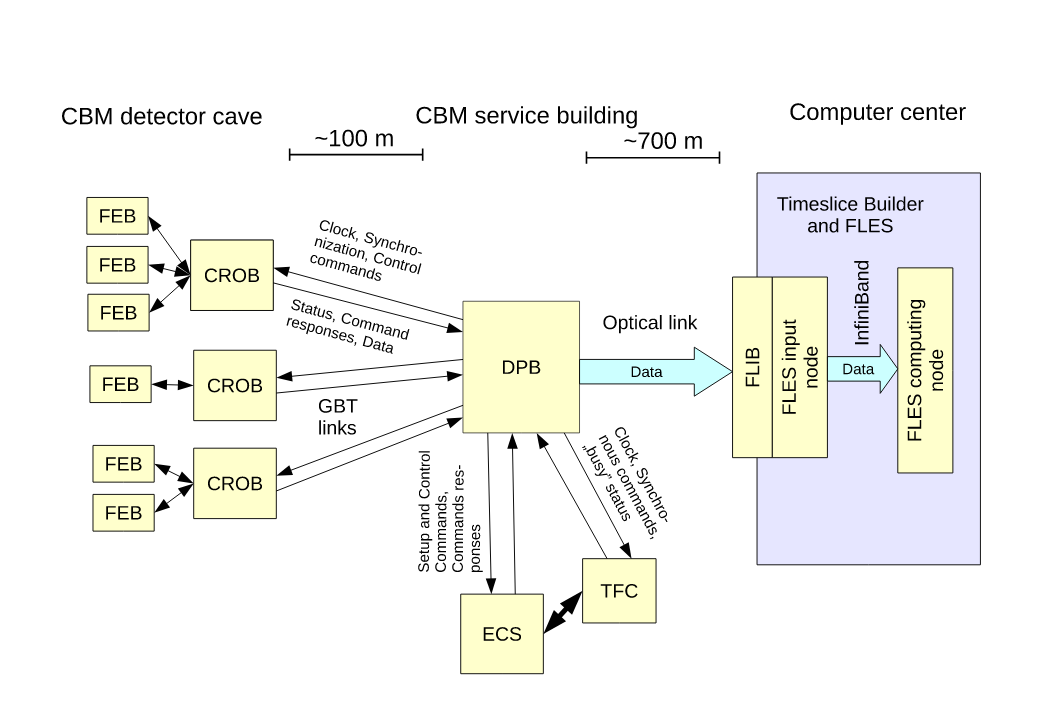
\includegraphics[width=0.75\columnwidth]{Chapter2/images/DPB.png}
\caption{The first proposition of the CBM readout chain based on separate DPB and FLIB boards \ref{fig_cri_board}}
\label{fig_dpb_scheme}
\end{figure}

\begin{figure}[!h]
\centering
\includegraphics[width=0.65\columnwidth]{Chapter2/images/feb_8_v2.pdf}
\caption{FEB}
\label{fig_febA_photo}
\end{figure}
\subsection{CRI based readout chain}
\begin{figure}[!h]
\centering
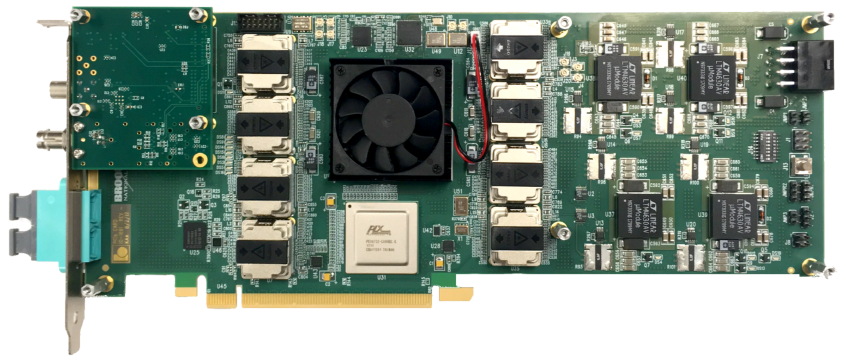
\includegraphics[width=0.65\columnwidth]{Chapter2/images/cri_board_atlas.pdf}
\caption{CRI board}
\label{fig_cri_board}
\end{figure}

\label{tester}
Another alternative to the two readout chains introduced in the last two sections is the so-called GBTxEMU-based tester. It is based on a commercial Artix-7 board (TE-0712, Trenz Electronics Gmbh), and allows emulating GBTX ASIC or the whole CROB. Moreover, it could also be used in an autonomous mode with the addition of VITA  57.1 FMC adapter
\subsection{Powering schematics of the detector}
\label{powering}
\subsection{Cooling concept for the STS's electronics and silicon sensors}
\label{cooling}

\subsection{Detector enclosure and its importance}
\section{System safety and the consequences}
\subsection{Requirements for the control system}
\label{sys:req}
Custom solutions that are applied in \gls{STS} make the control of this system very challenging. Different services imply different control solutions which need to be implemented.
A distributed control system should offer remote control, alarm detection, reporting and logging, modeling and simulation, data processing (archiving, retrieval, plotting, conversion, analysis), common time management, access security, and automatic \footnote{Sequencing, also known as sequential control, it controls the device in a pre-determined order.}{sequencing}.
In addition to that, the \gls{DCS} for the Silicon Tracking System (\gls{STS}) is being designed taking into consideration the following aspects:

 
 \begin{itemize}
    \item potential control framework should offer the possibility to control a variety of different services, which often have different communication protocols,
    \item logging, and monitoring - there should be reliable means of supervision of processes, containers, and \footnote{The input/output controller is a device that interfaces between an input or output device and the computer or hardware device}{Input/Output Controllers} (\glspl{IOC}).
    \item the control software should be horizontally and vertically scalable, when it comes to adding additional computing nodes or applications/Input Output Controllers (\glspl{IOC})/containers,
    \item supervision - it should be possible to integrate a sub-system oriented with higher-level control structures,
     \item flexible - applications should be easy to run on different operating systems and processor architectures,
     \item sustainability and support - the experiment is supposed to run for about 10 years, excluding the building and commissioning time. The control system should be sustainable and long-term support provided,
     \item reliability - the system should be highly available, minimizing the downtimes,
     \item network separation - it should be running in a dedicated network (divided into several service-oriented subnets) to have a good overview of the processes and communication between the nodes,
     \item \glspl{GUI} - all parameters/\footnote{In control theory, a process variable is the currently measured value of a particular part of a process which is being monitored or controlled}{process variables} should be available in a user-friendly Graphical User Interface (\gls{GUI}). In case of error or malfunction, it should be stated clearly by the software where the error happened, what could be the potential risk and what actions need to be taken.

 \end{itemize}
\newpage

